\chapter{Results}
\section{Overview}
Ground truth gathering was conducted over a two week period between 31/03/25 and 13/04/25. Data from \textit{04/04/25 - 11/04/25} for Israel and \textit{07/04/25 - 12/04/25} in the case of Ireland were exported for comparison and analysis. The results are discussed below, with pertinent tables included in the 'Appendix' section. In comparison, the publicly available OONI database was analysed for the dates 13/03/25 to 13/04/25. 

It is important to recognize that, particularly in the case of Israel, different individuals may experience censorship of the Internet to varying degrees. The research focuses on replicating the experience of the average Israeli living in Tel Aviv. Having previously discussed the Gaza Strip, it is clear that the user experience varies greatly between the two areas. Further research may look at comparing Internet censorship experienced internally in Israel, but that is outside the scope of this work.

In the following section, the relevant context regarding the network conditions while gathering ground truth will be discussed. Having previously highlighted the varying levels at which internet censorship can be conducted, let us now define the specific network characteristics under which the OONI probe was run for both countries.

\subsection{Network Environment Context: Ireland}
As mentioned, the OONI CLI probe is running on a Raspberry Pi 5, connected over WiFi to a home residential network. The provider is Virgin Media (AS12388), registered under Liberty Global B.V. ISP (AS6830). 

Details regarding the operating system flashed to the Raspberry Pi and packages required for this are illustrated below in the 'Guide to Replicating Results.' 

\subsection{Network Environment Context: Israel}
Ground truth gathering in Israel was done using a virtual machine as described in the section on methodology. The virtual machine is operates within a data center hosted by O.M.C. COMPUTERS \& COMMUNICATIONS LTD (AS44709), downstream of its owner Kamatera Inc. (AS36007). This differs from the residential network that is being tested in Ireland.


\section{Website Connectivity Tests}


\subsection{Ground Truth via SSH}
\subsection{Native Website Connectivity Tests}
This section details the results of the daily web connectivity tests performed using the command \textit{ooniprobe run}. 

\begin{table}[H]
\centering
\caption{Summary of Tested vs. Blocked Websites by Country (Native to OONI probe CLI)}
\begin{tabular}{lcc}
\toprule
\textbf{Country} & \textbf{Tested} & \textbf{Blocked} \\
\midrule
Ireland & 1695 & 25 \\
Israel    & 1695 & 16 \\   
\bottomrule
\end{tabular}
\label{tab:blocked_summary}
\end{table}




\subsection{my-websites.txt}
This file contains the additional 170 website connectivity tests I wished to conduct. The list was compiled with Griffin Steinman, and additional tests relating to Israel were added. The contents can be found within the Appendix section. Below is a summary of the results from the daily running of this additional web connectivity test suite.

\begin{table}[H]
\centering
\caption{Summary of Blocked vs. Unblocked Websites by Country (my-websites)}
\begin{tabular}{lcc}
\toprule
\textbf{Country} & \textbf{Unblocked} & \textbf{Blocked} \\
\midrule
Ireland & 151 & 19 \\
Israel    & 155 & 15 \\   
\bottomrule
\end{tabular}
\label{tab:blocked_summary}
\end{table}

The following figure illustrates the blocking methods for the additional web connectivity tests. See Appendix section for a more detailed breakdown of positive results for each locale.

\begin{table}[H]
\centering
\caption{Distribution of Blocking Methods Detected in Ireland \&Israel}
\begin{tabular}{lcc}
\toprule
\textbf{Blocking Method} & \textbf{Ireland} & \textbf{Israel} \\
\midrule
TCP/IP         & 15 & 13 \\
DNS            & 1  & 1  \\
HTTP           & 1  & 1  \\
Error/Failure  & 3  & 0  \\
\bottomrule
\end{tabular}
\label{tab:blocking_methods_comparison}
\end{table}

\begin{table}[H]
\centering
\caption{Blocked Websites by Category and Country}
\begin{tabular}{lccc}
\toprule
\textbf{Category} & \textbf{Total Websites Tested} & \textbf{Ireland} & \textbf{Israel} \\
\midrule
Uncategorized                      & 34 & 4 & 4 \\
Piracy / Streaming / File Sharing  & 21 & 6 & 4 \\
News / Media                       & 34 & 1 & 0 \\
Adult Content                      & 21 & 0 & 0 \\
Creative / Educational / Misc      & 15 & 1 & 1 \\
General / National Services        & 19 & 1 & 1 \\
Streaming / Social Media           & 9  & 0 & 0 \\
Religious                          & 5  & 2 & 2 \\
VoIP / Communication               & 4  & 1 & 0 \\
Gambling                           & 2  & 1 & 1 \\
Email/Privacy Tools                & 3  & 1 & 0 \\
Adult / Alcohol                    & 2  & 1 & 1 \\
LGBTQ+                             & 1  & 1 & 1 \\
AI / Technology                    & 1  & 0 & 0 \\
\bottomrule
\end{tabular}
\label{tab:category_block}
\end{table}

\subsection{Investigating Aljazeera.com}
Upon initial testing of Aljazeera URLs using the virtual machine in Israel, it was surprising to see no evidence of blocking. To investigate further it was decided that the content of the site should be examined and a variety of URLs belonging to it should be tested. Particular attention was given to articles that were critical of Israel. 

The file sample\_aljazeeraurls.txt contains 100 URLs for articles hosted on https://aljazeera.com. Below are some helpful commands used to obtain the sitemap and extract URLs for testing. Wget was used to examine the contents of the web page, and the following was observed.

Aljazeera and its articles were not found to be blocked on AS44709. Despite large ASNs consistently blocking connections, no evidence of this was found while testing O.M.C. COMPUTERS \& COMMUNICATIONS LTD (AS44709).

\begin{figure} [H]
    \centering
    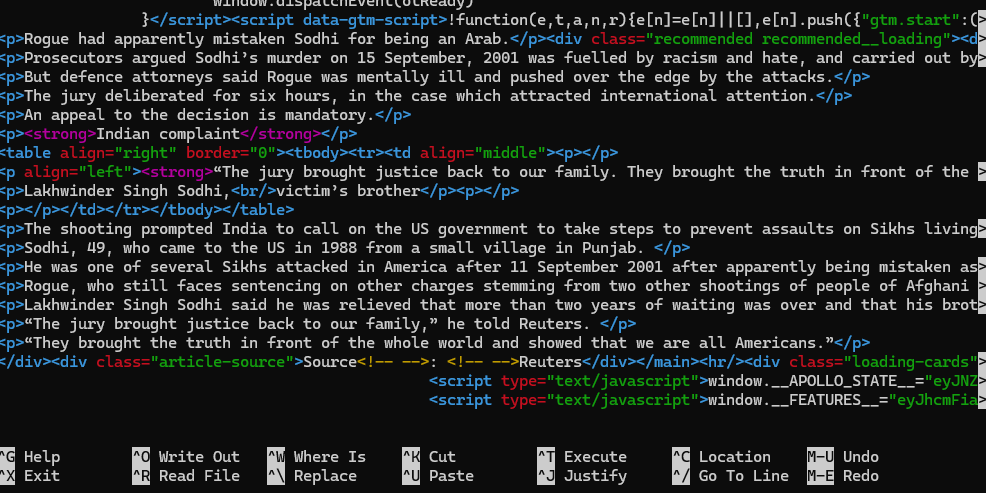
\includegraphics[width=1\linewidth]{wgetAljazeera.png}
    \caption{wget showing aljazeera.com content}
    \label{fig:enter-label}
\end{figure}


As seen above, I was able to see unblocked content from the site. Within Appendix, one can find a sample of articles being tested. 

\subsection{Public OONI Database}
In this section, the OONI database will be explored. As mentioned previously the period to be considered is 13/03/25 to 13/04/25. Below are screenshots of all web connectivity tests conducted in Ireland and Israel for these dates. 

By examining the publicly available data on Aljazeera and filtering based on ASN, an interesting picture emerges. There is clear evidence of large scale DNS tampering on certain ASNs, while others go unblocked. Prior to my testing using the VM in Tel Aviv, it was unknown whether O.M.C. COMPUTERS \& COMMUNICATIONS LTD (AS44709) was blocking this content. 

\begin{figure} [H]
    \centering
    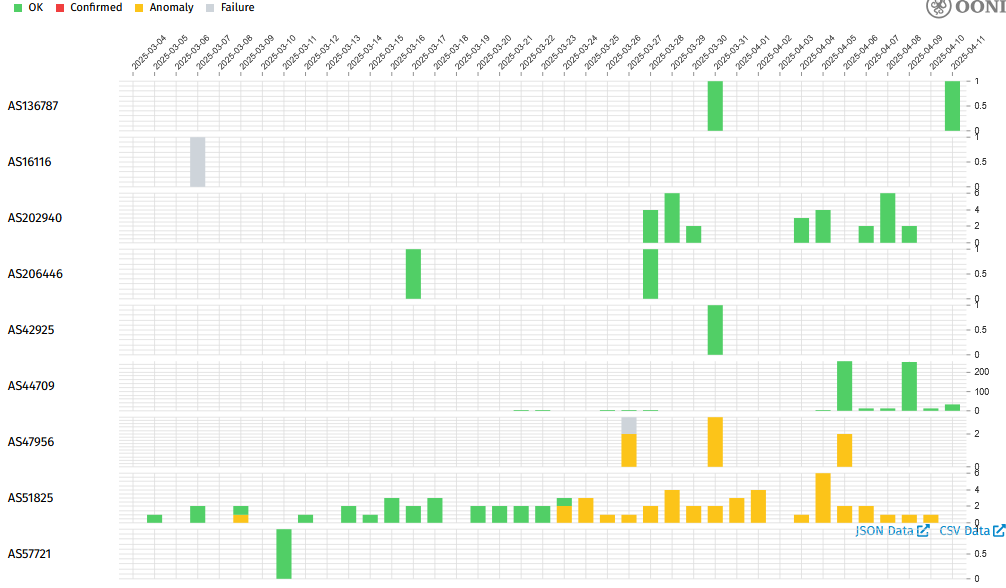
\includegraphics[width=1\linewidth]{ALJZRbyASN.png}
    \caption{OONI data (04/03/2025 - 11/04/2025) showing blocking of Alazeera.com grouped by ASN}
    \label{fig:enter-label}
\end{figure}

\begin{figure} [H]
    \centering
    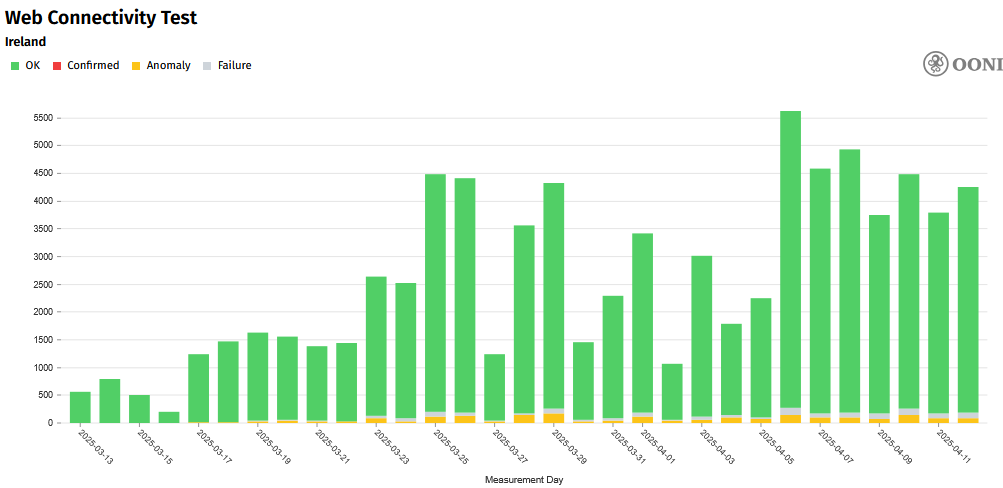
\includegraphics[width=1\linewidth]{IREWEBSOONIDB.png}
    \caption{Irish OONI Database Web connectivity tests 13/03-13/04}
    \label{fig:enter-label}
\end{figure}

\begin{figure} [H]
    \centering
    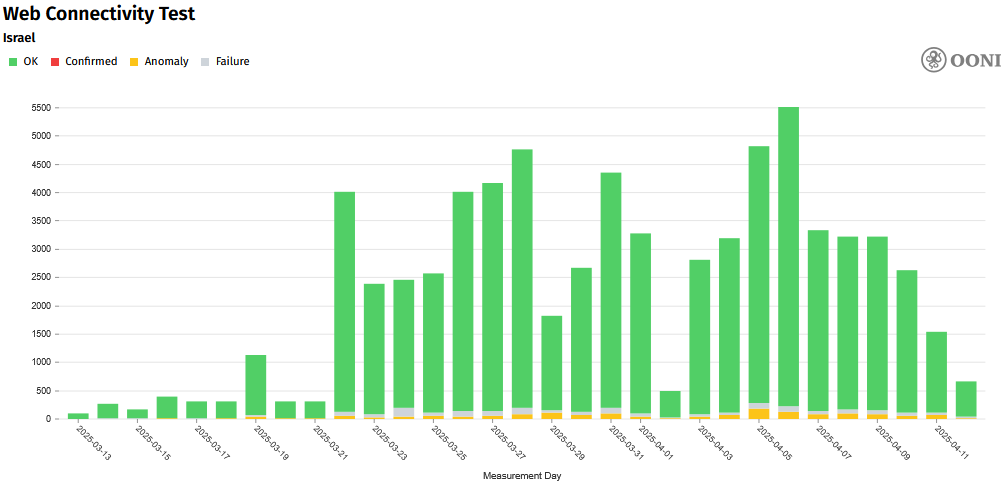
\includegraphics[width=1\linewidth]{ISRWEBSOONIDB.png}
    \caption{Israel OONI Database Web connectivity tests 13/03-13/04}
    \label{fig:enter-label}
\end{figure}

Further insight into this data can be seen through the proceeding table that documents a daily averages. 

\begin{table} [H]
\centering
\caption{Website Blocking based on Public OONI Data}
\begin{tabular}{lcc}
\toprule
\textbf{Metric} & \textbf{Ireland} & \textbf{Israel} \\
% \midrule
Number of Websites Tested           & 2603 &  2299 \\
Number of Successful Connections    & 2491 & 2195 \\
Number of Anomalies                 & 67 & 53 \\
Number of Failures                  & 46 & 51 \\
\bottomrule
\end{tabular}
\label{tab:category_block}
\end{table}


\section{Instant Messaging Tests}
By analysing the publicly available OONI data for both countries for the period of interest we can see little evidence of blocking of instant messaging platforms in either country.

\subsection{Public OONI Database: Ireland}
As seen in the below figures, there is little evidence to suggest network interference of instant messaging platforms in Ireland over the period considered.

\begin{figure} [H]
    \centering
    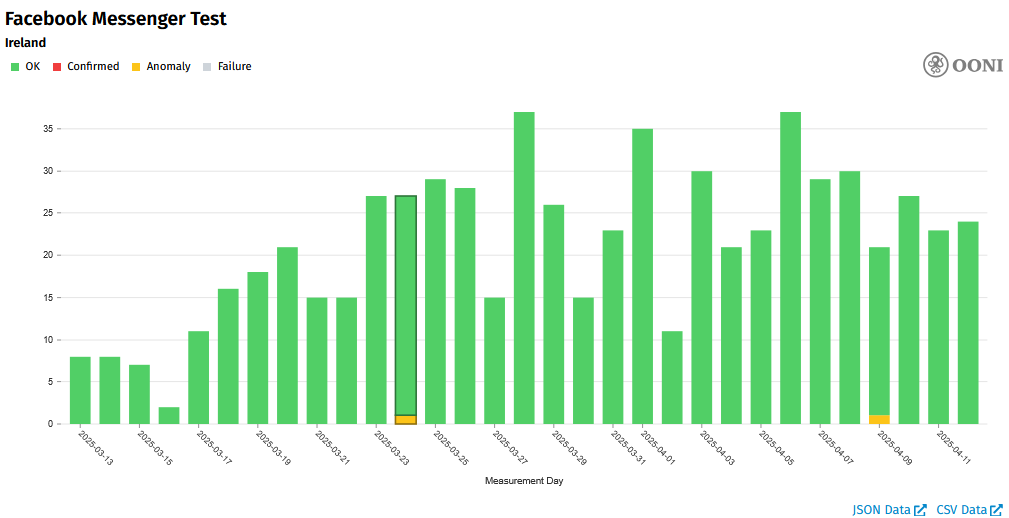
\includegraphics[width=0.5\linewidth]{IREOONIDBIMFB.png}
    \caption{Facebook Messenger test results for Ireland 13/03-13/04}
    \label{fig:enter-label}
\end{figure}

\begin{figure} [H]
    \centering
    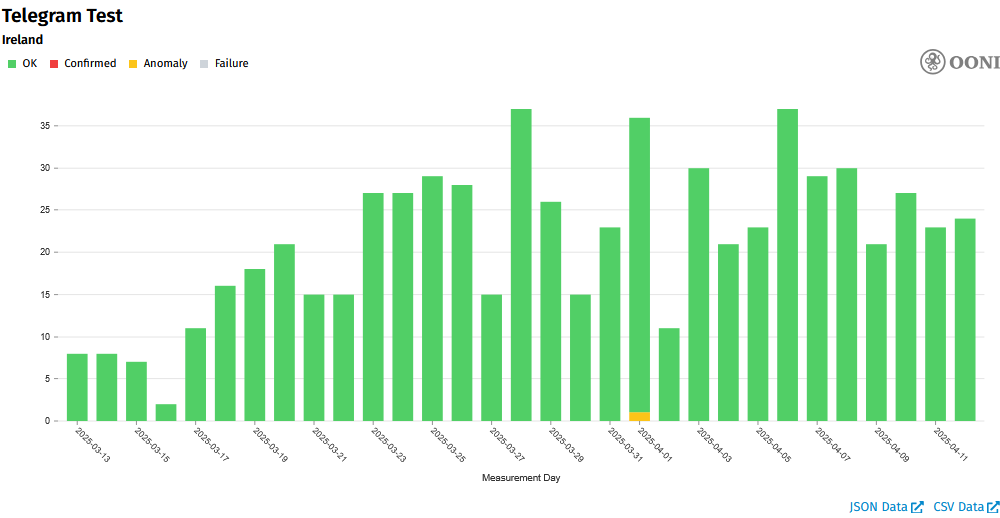
\includegraphics[width=0.5\linewidth]{IREOONIDBIMTL.png}
    \caption{Telegram test results for Ireland 13/03-13/04}
    \label{fig:enter-label}
\end{figure}

\begin{figure} [H]
    \centering
    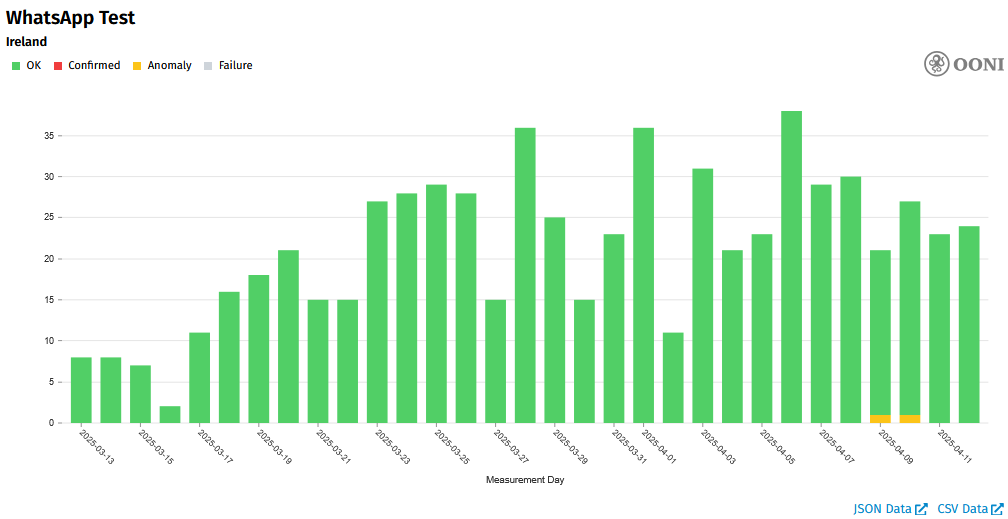
\includegraphics[width=0.5\linewidth]{IREOONIDBIMWHATS.png}
    \caption{WhatsApp test results for Ireland 13/03-13/04}
    \label{fig:enter-label}
\end{figure}

\begin{figure} [H]
    \centering
    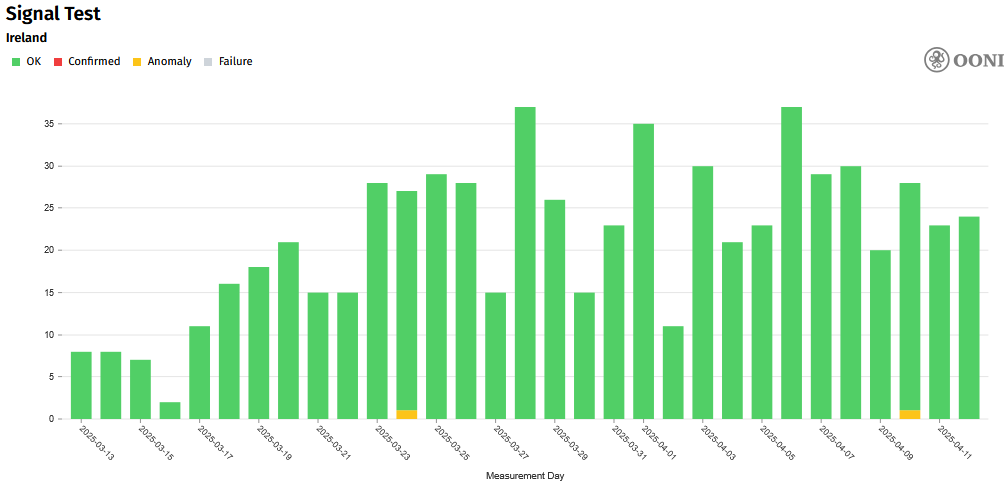
\includegraphics[width=0.5\linewidth]{IREOONIDBSIG.png}
    \caption{Signal test results for Ireland 13/03-13/04}
    \label{fig:enter-label}
\end{figure}



\subsection{Public OONI Database: Israel}
As seen in the below figures, there is little evidence to suggest network interference of instant messaging platforms in Israel over the period considered.

\begin{figure} [H]
    \centering
    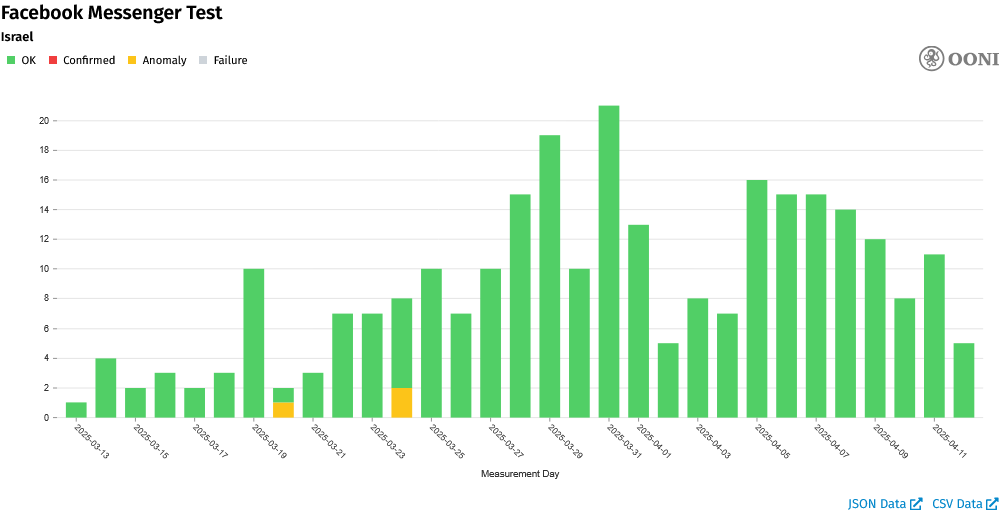
\includegraphics[width=0.5\linewidth]{ISROONIDBFB.png}
    \caption{Facebook Messenger test results for Israel 13/03-13/04}
    \label{fig:enter-label}
\end{figure}
\begin{figure} [H]
    \centering
    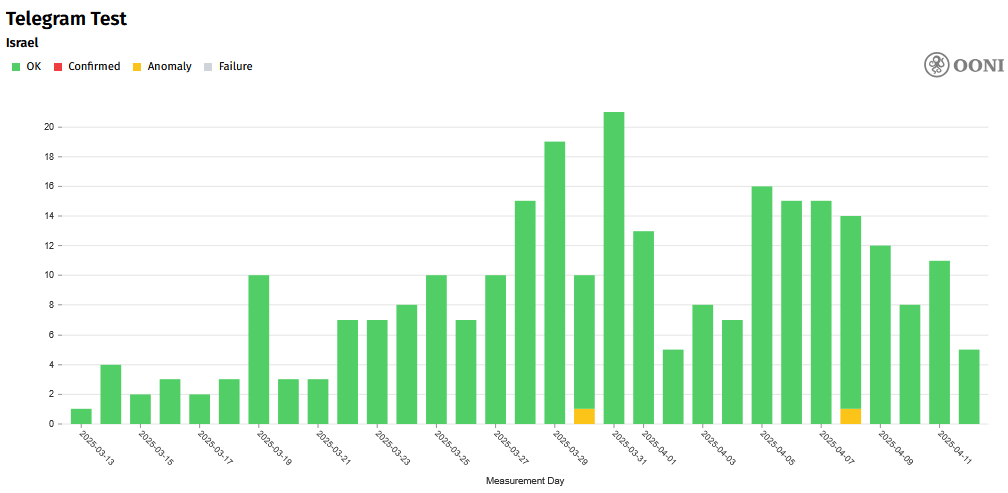
\includegraphics[width=0.5\linewidth]{ISROONIDBIM.png}
    \caption{Telegram test results for Israel 13/03-13/04}
    \label{fig:enter-label}
\end{figure}
\begin{figure} [H]
    \centering
    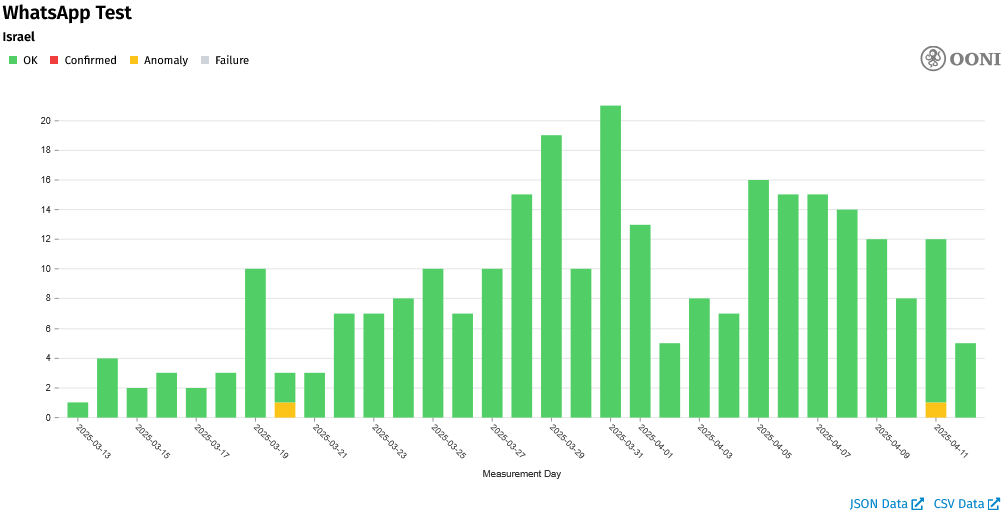
\includegraphics[width=0.5\linewidth]{ISROONIDBTEL.png}
    \caption{WhatsApp test results for Israel 13/03-13/04}
    \label{fig:enter-label}
\end{figure}
\begin{figure} [H]
    \centering
    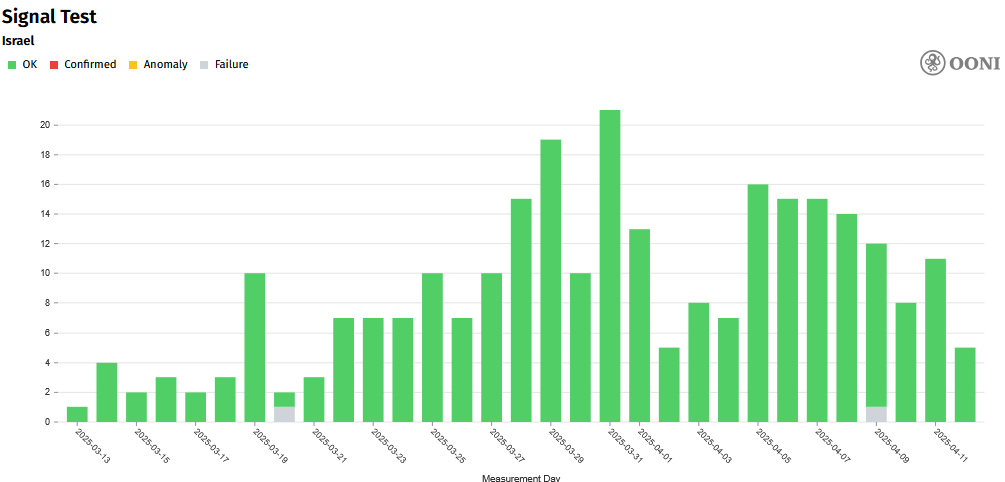
\includegraphics[width=0.5\linewidth]{ISROONIDBSIG.png}
    \caption{Signal test results for Israel 13/03-13/04}
    \label{fig:enter-label}
\end{figure}


\subsection{Ground Truth via SSH}
While running tests locally, no evidence for the blocking of instant messaging platforms was found in either Ireland or Israel. As seen in the above figures, there is little evidence in the OONI database to suggest either country interferes with instant messaging platforms. 


\section{Circumvention Tests}
\subsection{Public OONI Database: Ireland}

The majority of circumvention tests go unblocked in Ireland, however, certain ASNs show evidence of blocking. This can be see below.

\textbf{Ireland Circumvention Test Anomalies}
Based on data seen in the OONI database, TOR is not blocked by the majority of ASNs in Ireland. However, consistent blocking is seen in some networks. Over the period considered, there were seven instances of TOR being blocked, all attributed to HEAnet (AS 1213).

Psiphon appears to be blocked somewhat consistently on certain ASNs. The results are seen tabulated below, with a focus on ASNs containing anomalies.

\begin{table}[H]
\centering
\caption{Psiphon Circumvention Anomalies in Ireland}
\begin{tabular}{lccc}
\toprule
\textbf{Metric / ASN} & \textbf{Blocked} & \textbf{OK} & \textbf{\% Blocked} \\
\midrule
\textbf{Total}     & 82  & 575 & 12.48\% \\
\midrule
ASN 1213           & 57  & 6   & 90.48\% \\
ASN 6830           & 18  & 271 & 6.23\% \\
ASN 13280          & 5   & 13  & 27.78\% \\
ASN 9009           & 1   & 6   & 14.29\% \\
ASN 212238         & 1   & 0   & 100.00\% \\
ASN 8075           & 1   & 0   & 100.00\% \\
ASN 15751          & 1   & 8   & 11.11\% \\
\bottomrule
\end{tabular}
\label{tab:psiphon_ireland}
\end{table}



\begin{figure} [H]
    \centering
    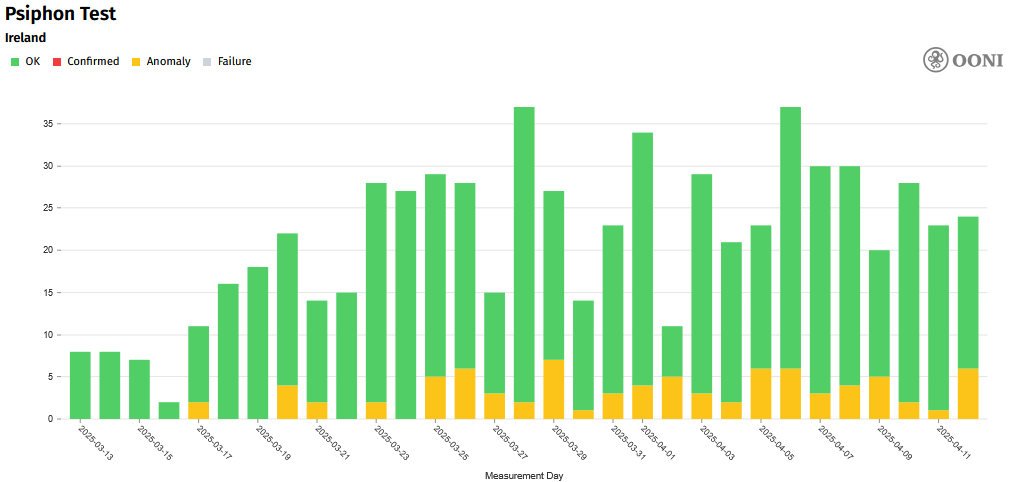
\includegraphics[width=0.5\linewidth]{IREDBPSI.png}
    \caption{Psiphon test results for Ireland 13/03-13/04}
    \label{fig:enter-label}
\end{figure}

\begin{figure} [H]
    \centering
    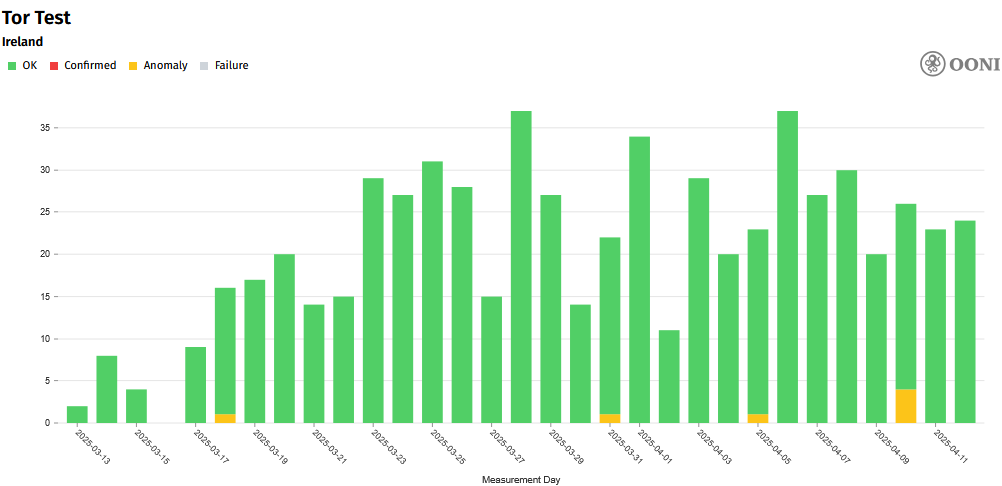
\includegraphics[width=0.5\linewidth]{IREDBTOR.png}
    \caption{TOR test results for Ireland 13/03-13/04}
    \label{fig:enter-label}
\end{figure}

\subsection{Public OONI Database: Israel}

Based on observations of the OONI database over the period of interest, TOR and Psiphon tests are not blocked in Israel. The only evidence of blocking comes from one autonomous system as described below.

\textbf{Israel Circumvention Test Anomalies}
ITC NG ltd (AS 202940) was responsible for 25 instances of blocking TOR connections and one instance of blocking Psiphon connections over the dates examined. This was the only ASN repsponsible for positive results. These anomalies are tabulated below.

\begin{table}[H]
\centering
\caption{Circumvention Results in Israel (ASN 202940)  (13/03-13/04)}
\begin{tabular}{lccc}
\toprule
\textbf{Tool} & \textbf{Blocked (Anomaly)} & \textbf{OK} & \textbf{\% Blocked} \\
\midrule
Psiphon & 1  & 27 & 3.57\% \\
Tor     & 25 & 3  & 89.29\% \\
\bottomrule
\end{tabular}
\label{tab:circumvention_israel}
\end{table}


\begin{figure} [H]
    \centering
    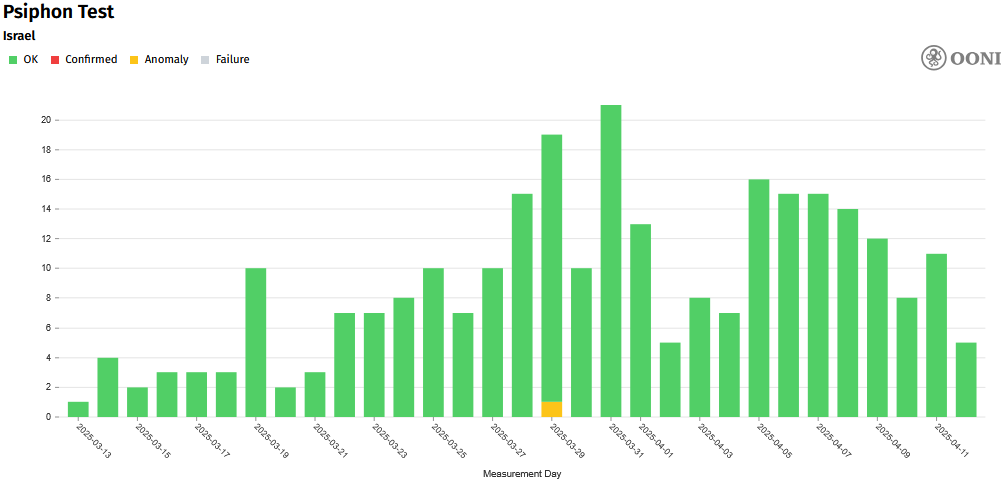
\includegraphics[width=0.5\linewidth]{ISROONIPSI.png}
    \caption{Psiphon test results for Israel 13/03-13/04}
    \label{fig:enter-label}
\end{figure}

\begin{figure} [H]
    \centering
    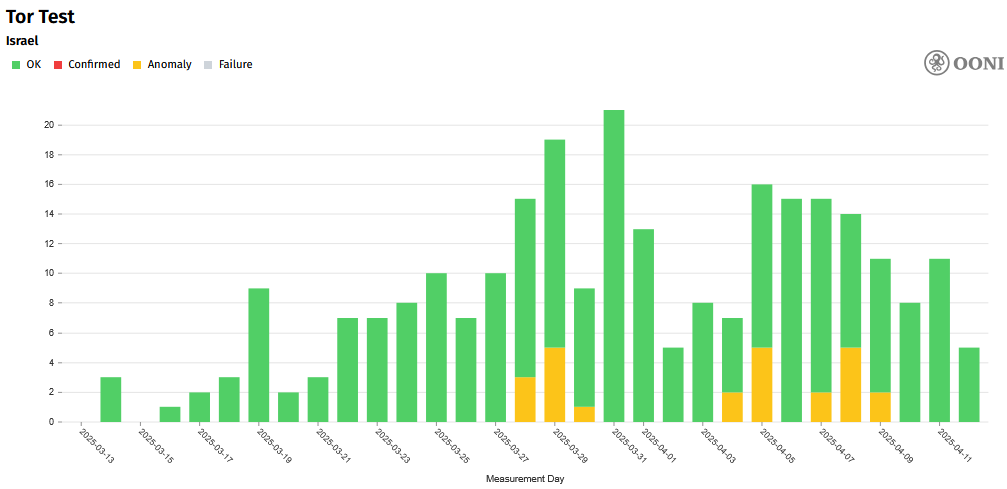
\includegraphics[width=0.5\linewidth]{ISROONITOR.png}
    \caption{TOR test results for Israel 13/03-13/04}
    \label{fig:enter-label}
\end{figure}

\subsection{Ground Truth via SSH}
No evidence for the blocking of TOR or Psiphon was found while running circumvention tests in either locale. This is consistent with the OONI database as in both countries, blocking appears inconsistent and AS specific.



\section{Middlebox Tests}
\subsection{Public OONI Database: Ireland}
In examining the OONI database for HTTP Invalid Request Line tests conducted in Ireland over the period of interest, only a handful of anomalies are observed. Out of the 660 HTTP Invalid Request Line tests conducted there were 5 anomalies. These instances belonged to M247 Europe SRL (AS9009), Vodafone Ireland Limited (AS15502) and Meteor Mobile Communications Limited (AS15751). A breakdown of the anomalies is seen below.

\begin{table}[H]
\centering
\caption{HTTP Invalid Request Line Test Anomalies in Ireland (13/03-13/04)}
\begin{tabular}{lcc}
\toprule
\textbf{ASN} & \textbf{Anomalies} & \textbf{OK} \\
\midrule
\textbf{Total}   & 5 & 660 \\
\midrule
AS9009           & 3 & 4 \\
AS15502          & 1 & 103 \\
AS15751          & 1 & 9 \\
\bottomrule
\end{tabular}
\label{tab:http_invalid_ireland}
\end{table}



\begin{figure} [H]
    \centering
    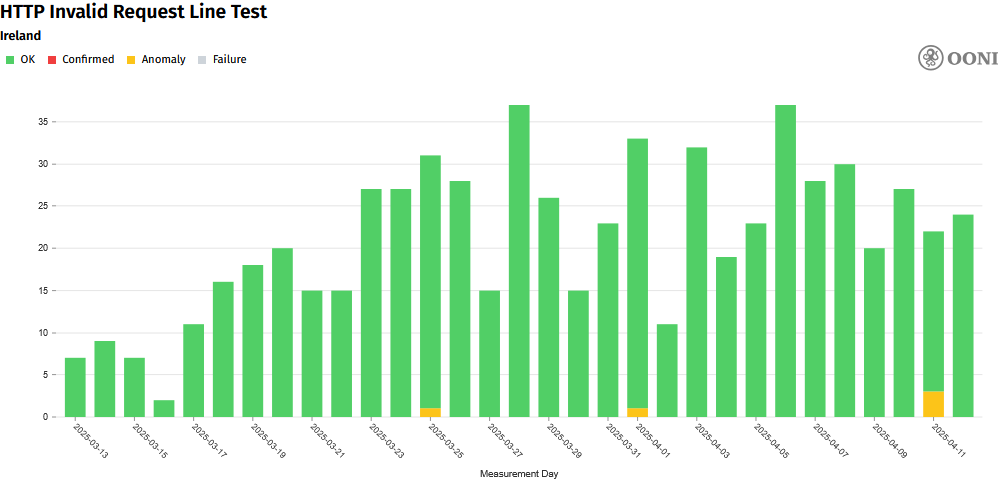
\includegraphics[width=0.5\linewidth]{IREOONIDBMB1.png}
    \caption{HTTP Invalid Request test results for Ireland 13/03-13/04}
    \label{fig:enter-label}
\end{figure}

Irish tests for HTTP Header Field Manipulation were less intriguing with only 6 anomalies over the period of interest. These were attributed to M247 Europe SRL (AS9009) and HEAnet (AS 1213) respectively. A breakdown of these results is seen below.


\begin{table}[H]
\centering
\caption{HTTP Header Field Manipulation Anomalies in Ireland}
\begin{tabular}{lccc}
\toprule
\textbf{ASN} & \textbf{Anomalies} & \textbf{OK} & \textbf{Percentage Anomalous} \\
\midrule
\textbf{Total}   & 6 & 648 & 0.91\% \\
\midrule
AS9009           & 2 & 1   & 66.67\% \\
AS1213           & 4 & 7   & 36.36\% \\
\bottomrule
\end{tabular}
\label{tab:http_header_ireland}
\end{table}

\begin{figure} [H]
    \centering
    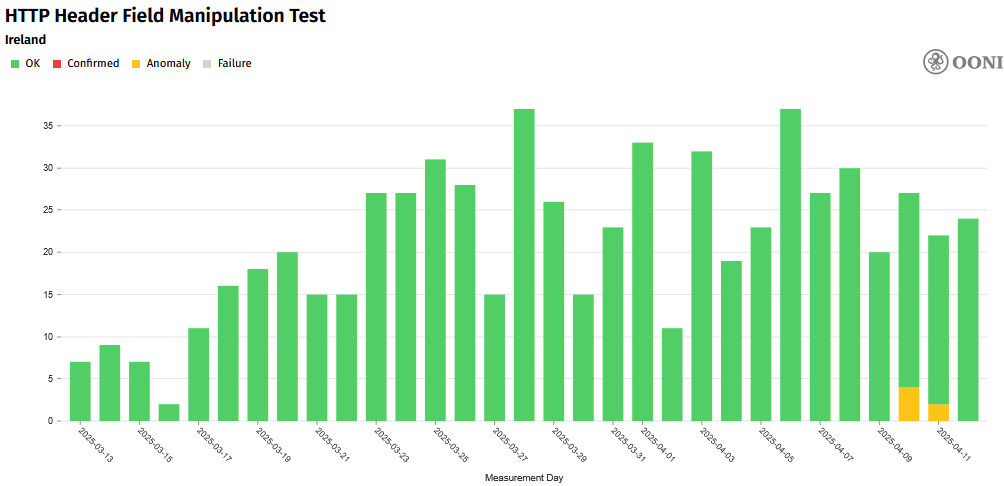
\includegraphics[width=0.5\linewidth]{IREOONIDBMB2.png}
    \caption{HTTP Header Field Manipulation test results for Ireland 13/03-13/04}
    \label{fig:enter-label}
\end{figure}


\subsection{Public OONI Database: Israel}
Only one instance of HTTP a Invalid Request Line anomaly was seen in Israel over the period of interest and belonged to XFone 018 Ltd (AS47956). 


\begin{figure} [H]
    \centering
    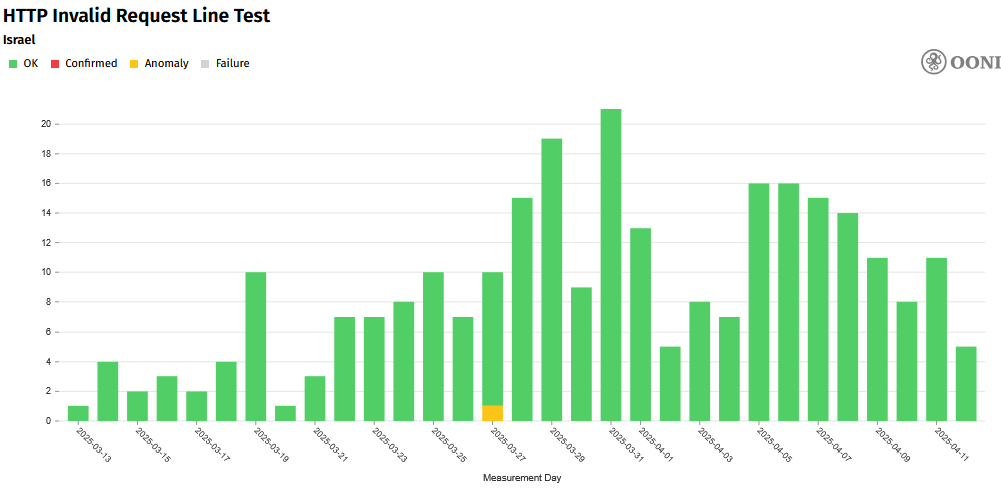
\includegraphics[width=0.5\linewidth]{ISROONIDBMB1.png}
    \caption{HTTP Invalid Request test results for Israel 13/03-13/04}
    \label{fig:enter-label}
\end{figure}

On the other hand, HTTP Header Field Manipulation test results for Israel were quite interesting. Anomalies were attributed to three different ASNs: Cellcom Fixed Line Communication L.P (AS1680), ITC NG ltd (AS202940) and XFone 018 Ltd (AS47956). The breakdown of these results is tabulated below.

\begin{table}[H]
\centering
\caption{HTTP Header Field Manipulation Anomalies in Israel}
\begin{tabular}{lccc}
\toprule
\textbf{ASN} & \textbf{Anomalies} & \textbf{OK} & \textbf{Percentage Anomalous} \\
\midrule
\textbf{Total}       & 35 & 237 & 12.87\% \\
\midrule
AS202940             & 25 & 4   & 86.21\% \\
AS1680               & 9  & 3   & 75.00\% \\
AS47956              & 1  & 7   & 12.50\% \\
\bottomrule
\end{tabular}
\label{tab:http_header_israel}
\end{table}


\begin{figure} [H]
    \centering
    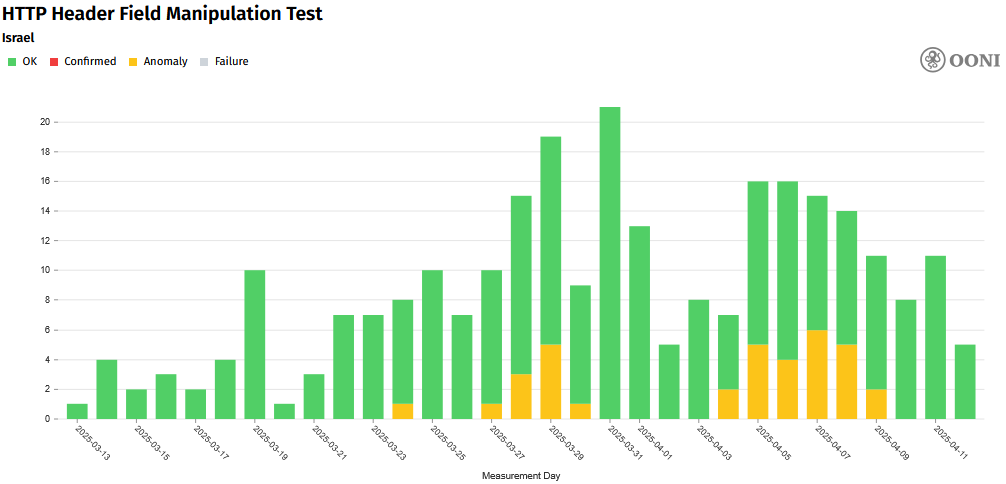
\includegraphics[width=0.5\linewidth]{ISROONIDBMB2.png}
    \caption{HTTP Header Field Manipulation test results for Israel 13/03-13/04}
    \label{fig:enter-label}
\end{figure}

\subsection{Ground Truth via SSH}
Results of running middlebox tests locally in both countries showed no evidence of tampering of presence of middleboxes. However, as seen above Cellcom Fixed Line Communication L.P (AS1680) and ITC NG ltd (AS202940) are responsible for a significant number of positive with a majority of the measurements conducted on their networks showing interference. 

\section{Comparative Analysis: Ireland vs. Israel}
The objective of this section is to summarise key findings from the research conducted. This is done in the context of ground truth gathered and the publicly available OONI database. Particular attention is given to positive results, showing evidence of network interference. False positives can occur and as a result, consistent trends will hold more weight.



\subsection{Websites}
\large\textbf{Ireland}
Ground truth testing in Ireland demonstrated relatively low levels of website blocking. The vast majority of websites loaded successfully across multiple test runs. Public OONI data corroborated this finding, showing a low anomaly rate with most anomalies appearing as isolated incidents rather than persistent patterns. 

Contrastingly, consistent blocking of piracy websites such as torrents or \textit{thepiratebay.org} was observed. This was in line with expectations based on the research conducted on Irish and European law during the literature review.

\large\textbf{Israel}
Results from running the curated \textit{my-websites} and the native OONI URL suite were similar across both countries. Slightly lower rates of censorship were observed in the case of Israel. OONI public data shows that Ireland had 2,491 successful web connectivity tests out of the 2,603 conducted between 13/03 and 13/04. Israel had 2,195 successful web connectivity tests out of the 2,299 conducted between 13/03 and 13/04.

\subsection{Instant Messaging}
\large\textbf{Ireland}
Tests on instant messaging platforms such as WhatsApp, Facebook Messenger, and Telegram showed no trends of being blocked. All IM services functioned as expected during ground truth gathering, and the OONI database results for Ireland showed only a handful of anomalies between 13/03 and 13/04.

\large\textbf{Israel}
Similarly, Israeli networks did not show blocking of mainstream messaging platforms in either ground truth data or public OONI records. Tests confirmed that services like WhatsApp and Signal were reachable and functional without evidence of throttling or manipulation, aside from a handful of anomalies throughout the month of interest.

\subsection{Circumvention Tools}
\large\textbf{Ireland}
Blocking was observed in Psiphon test results, particularly on ASN 1213 (HEAnet CLG), where a significant number of anomalies were noted. This ASN is associated with institutes of education. This contrasted with the residential setting where ground truth was gathered in which Psiphon operated without issue. Public OONI data supported these observations, indicating selective blocking by ASN. Tor tests, however, showed minimal interference across all networks.

\large\textbf{Israel}
The Israeli results stood out due to clear and persistent blocking of circumvention tools. Psiphon exhibited an anomaly rate of nearly 4\%, with a single confirmed block found on ITC NG ltd. (AS202940). Tor network usage on this particular ASN faced significant restrictions, with nearly 90\% of Tor test runs resulting in anomalies. Outside of this case, blocking of circumvention methods was sparse.

\subsection{Middleboxes}
\large\textbf{Ireland}
No middlebox interference was detected during ground truth gathering in Ireland. Both ground truth and OONI public results consistently showed  little evidence to suggest middlebox presence. The OONI database shows 660 successful 'HTTP Invalid Request Line' test instances with only 5 anomalies attributed to a three ASNs, (Meteor (AS15751), Vodafone (AS15502) and M247 Europe(AS9009)). It is interesting to note the two mobile carriers showing positive results for this test.

'HTTP Header Field Manipulation' tests conducted in Ireland across the period of interest also showed no evidence of middlebox presence, outside of two Autonomous Systems. M247 Europe(AS9009) and HEAnet CLG AS1213 (AS1213) had percentage anomalies of 66.67\% and 36.36\% respoectively, though the test sample is small.

\large\textbf{Israel}
Israel presented similar results for 'HTTP Invalid Request Line' tests, with little concrete evidence of manipulation or network interference in this manner. Both local testing and the OONI database confirmed these results.

'HTTP Header Field Manipulation' tests on the other hand paint a different picture. Though no anomalies were found during local testing, ITC NG ltd. (AS20294) and Cellcom Fixed Line Communication L.P (AS1680) were shown to present anomalies in a majority of tests, 86.21\% and 75\% respectively. These anomalies accounted for 12.87\% of the header field manipulation tests conducted

\subsection{Conclusions: Ireland versus Israel}
While both countries show limited interference with messaging platforms, circumvention tools, middlebox presence and website connectivity tests reveal marked differences. While gathering ground truth, Ireland appeared to censor more content online. This could be attributed to the network description above. Speculating, the ASN in Israel could be more passive in its censoring due to the applications it serves (business solutions with less focus on consumers). 

Based on table 6.5 'Website Blocking based on Public OONI Data,' the number of anomalies and failures when testing websites is comparable. As in the table, 2603 URLs were tested with 67 anomalies and 46 failures in the case of Ireland, while 2299 URLs were tested with 53 anomalies and 51 failures in the case of Israel.

The results of the middlebox detection tests highlight a nuanced distinction between the two countries. In Ireland, the 'HTTP Invalid Request Line' and 'HTTP Header Field Manipulation' tests showed minimal evidence of middlebox interference. Out of 660 invalid request line tests, only 5 anomalies were observed, attributed to a small number of ASNs, including mobile carriers such as Meteor and Vodafone. Header manipulation tests yielded similar trends with isolated anomalies from AS9009 and AS1213, though the limited sample size tempers any strong conclusions. In contrast, Israel's 'HTTP Invalid Request Line' test results also revealed few anomalies, suggesting little evidence of systematic packet manipulation. However, the 'HTTP Header Field Manipulation' test results deviated significantly. AS202940 and AS1680 presented anomalies in 86.21\% and 75\% of cases respectively, pointing to a more assertive use of traffic modification techniques on select networks. This contrast may reflect policy differences in handling deep packet inspection or divergent technical implementations between ISPs.

A clear disparity emerges in the analysis of circumvention tool accessibility. In Ireland, Psiphon was selectively blocked, with anomalies primarily concentrated on HEAnet (AS1213), an ASN serving educational institutions. Residential networks, including that used in ground truth gathering, showed no evidence of Psiphon blocking, and Tor tests exhibited little to no interference across all networks. This indicates that censorship of circumvention tools in Ireland is limited. Meanwhile, Israeli networks, particularly ITC NG Ltd. (AS202940), demonstrated aggressive blocking behavior. Almost 90\% of Tor test instances resulted in anomalies, and Psiphon showed repeated anomalies with one confirmed block. These results suggest a more active censorship strategy employed on specific ASNs, while others remained largely permissive. Overall, certain Israeli ASNs appear to implement targeted blocking of circumvention technologies, contrasting with the sparse evidence seen in the case of Ireland.

\subsection{Further Research}
\textsc{Ireland}
As mentioned previously, ground truth gathering was conducted using a Raspberry Pi connected to a home network. In this way, the internet censorship experience of the average citizen was likely emulated during testing. Comparing results with Griffin Steinman, the other student partaking in the thesis, we see some discrepancy between internet censorship situation in residential networks and institutions (Trinity College Dublin). Based on the observed differences, this could be a compelling area of research; comparing the internet censorship situation experienced on residential and institutional networks. 

\textsc{Israel}
Highlighted above was the disparity between network interference observed in the ASN on which ground truth was gathered (O.M.C. COMPUTERS \& COMMUNICATIONS LTD, AS44709) and that observed by others. It was mentioned that the hosting provider \textit{(interhost.il)} is a data center. This begs the question: is the ground truth gathered representative of the average Israelite's experience online? This was bolstered by the Aljazeera case study, where a large volume of blocking was observed in other Autonomous Systems. Results gathered show less blocking across all categories when compared to popular consumer-used ASNs such as ITC NG ltd (AS202940) or Partner Communications Ltd. (AS12400). Below is OONI data regarding website blocking in Israel during 13/03-14/03, filtered by those ASNs to illustrate this. According to ipInfo \cite{ipinfo_israel_asns}, Partner Communications Ltd. (AS12400) owns the largest range of IPs in the country and was thus used for comparison.

A compelling area of further research may be the internet censorship experience of individuals of varying social identities. A difference in the censorship results between ASNs has been noted, however their consumer base has not been examined. I would speculate that, based on trends and events noted in the 'Literature Review' chapter, the Gaza Strip may be subject to inordinate internet censorship and surveillance. Especially when compared to Tel Aviv, where the VM was located.


\begin{figure} [H]
    \centering
    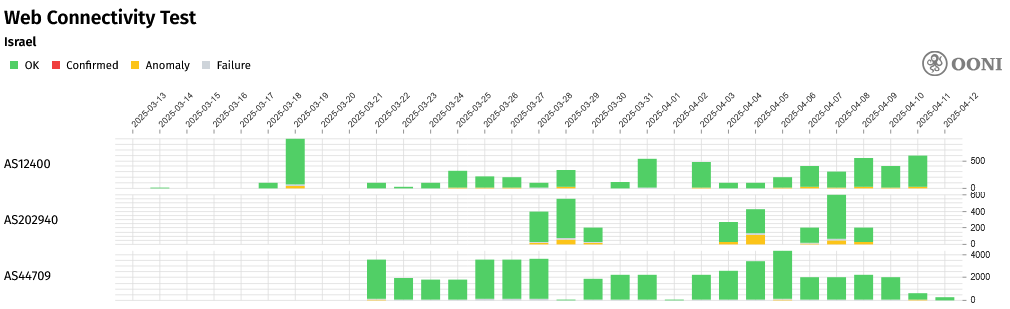
\includegraphics[width=1\linewidth]{ISRWEBASNcomp.png}
    \caption{Website Connectivity results for the ASN tested and two other popular providers in Israel during 13/03-13/04}
    \label{fig:enter-label}
\end{figure}


\section{Guide to Replicating Results}

\subsection{Investigating Aljazeera}
Below are some commands used to investigate \textit{https://aljazeera.com/}

\begin{figure} [H]
    \centering
    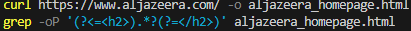
\includegraphics[width=0.5\linewidth]{AljazeeraURLs1.png}
    \caption{Using curl and grep to scrape URLs for articles}
    \label{fig:enter-label}
\end{figure}

\begin{figure} [H]
    \centering

\includegraphics[width=0.5\linewidth]{AljazeeraComs2.png}
    \caption{Inserting a dash after each URL, can now be ran with OONI}
    \label{fig:enter-label}
\end{figure}


\subsection{Raspberry Pi Setup}
\textbf{Operating System}
The operating system used was the latest available version of Raspberry Pi OS (64-bit) at the time of testing. It was flashed using the Raspberry Pi Imager application over USB. 

\begin{flushleft}
\hspace{1em}\textbf{Raspberry Pi OS (64-bit)}\\[0.5em]
\hspace{1em}Release date: November 19th 2024\\[0.5em]
\hspace{1em}System: 64-bit\\[0.5em]
\hspace{1em}Kernel version: 6.6\\[0.5em]
\hspace{1em}Debian version: 12 (bookworm)
\end{flushleft}


\textbf{Packages Installed}
In order to install the OONI probe CLI, the guide 'Install OONI Probe CLI on Debian/Ubuntu Linux' \cite{ooni-cli-install} was followed. The process was similar to that of installing on the Israeli VM. One obstacle faced in both instances were OpenPGP errors. To solve, the permissions for OONI probe had to be updated to bypass PGP signature verification. To do this, /etc/apt/sources.list.d/ooniprobe.list was edited to include '[trusted=yes]'

\begin{figure} [H]
    \centering
    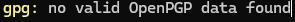
\includegraphics[width=0.5\linewidth]{PGPERROR.png}
    \caption{PGP Error installing CLI}
    \label{fig:enter-label}
\end{figure}


